\hypertarget{bells-future-quantum-mechanics---a-novel-interpretation}{%
\section{Bell's Future Quantum Mechanics - a Novel
Interpretation}\label{bells-future-quantum-mechanics---a-novel-interpretation}}

This essay provides an introduction to a new interpretation for quantum
mechanics. Here it is in two sentences:

\begin{verbatim}
Bell's inequality backed by experimental evidence shows that
quantum mechanics must be non-local, thus the wave function
is space-like separated from the observer at the origin, 
here-now. The product of the wave function and its conjugate
provide the odds for an interaction with the observer 
happening here (0, 0, 0) in the future.
\end{verbatim}

This novel interpretation is called Bell's future quantum mechanics.

\hypertarget{new-views-on-old-space-time}{%
\subsection{New Views on Old
Space-time}\label{new-views-on-old-space-time}}

Start with a Minkowski space-time graph. All information that is local
to the observer at the origin here-now is in the past lightcone. Quantum
mechanics is non-local, ergo delete all local information - delete the
past lightcone! The wave function has to reside in the space-like
regions of space-time. The conjugate of the wave function goes on the
other side. The product of the wave function and its conjugate is
necessarily in the future at the spatial origin (here, or (0, 0, 0)).
Quantum mechanics has always been about the future. What are the odds
that an event will happen to an observer in the future? Bell's
inequality is about the non-local nature of quantum mechanics. Deleting
the past lightcone enforces non-locality. Space-like information can be
used only to predict the future. This is the Bell's Future
interpretation of quantum mechanics.

\hypertarget{historical-background}{%
\subsection{Historical Background}\label{historical-background}}

In 1935, Einstein, Polodsky, and Rosen (EPR) proposed that variables
hidden in the past light cone could explain how quantum mechanics
worked. The claimed inherent uncertainty of quantum mechanics could be
traded for something more real, variables that are hidden. This was not
an easy to dismiss proposal given Einstein's stature. It took until the
1960s when John Bell found an inequality that could test if variables
are hidden in the past lightcone or the entangled states of quantum
mechanics where somehow real because quantum information was non-local.
If one asks the same question the same way, both models make identical
predictions. If questions are asked at a different angle, the hidden
variable hypothesis is unchanged. Quantum mechanics says correlations
between measurements become stronger. A huge experimental effort from
the 1980s until today has always confirmed the same result: quantum
mechanics is non-local and hidden variable models are wrong.

\hypertarget{my-beliefs-about-it-all-in-3d-space-time}{%
\subsection{My Beliefs About It All in 3D Space +
Time}\label{my-beliefs-about-it-all-in-3d-space-time}}

Einstein put Lorentz transformations to great use to solve difficult
theoretical problems in physics. It was his math professor who
recognized that Einstein was doing rotations not just in space, but in
space-time. Here is a picture of all of space:

\begin{figure}
\centering
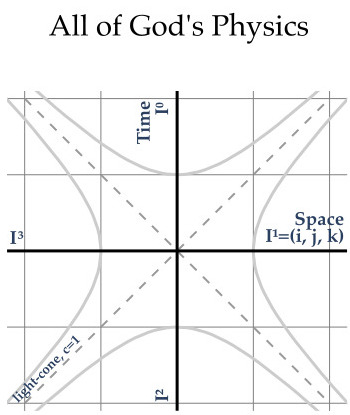
\includegraphics{../images/QM/BellsFuture/Bells_future_QM_all.jpg}
\caption{All of God's Physics}
\end{figure}

I hope the gentle reader is not offput by referencing a diety. The word
choice was made because it is my belief that all of physics, both that
that is currently known which is the vast majority, and that which
remain unknown, must live only in 3D space + time, or space-time. I am
more concerned with why parity is not conserved for beta decay than any
biblical issue.

Noice how three spatial dimensions are written explicity in the
space-time graph. Starting from studies done with five dimensions in the
1920s, research begun in the 1970s created a significant investigation
into higher spatial dimensions. I believe all such work will have no
lasting value. More recently, people have been championing the
multi-verse. A multi-verse has multiple space-times. Again, I believe
all such work witll have no lasting value.

I am radical conservative circa 1960s in regards to space-time.

\hypertarget{technical-tangent-quaternions}{%
\subsubsection{Technical Tangent:
quaternions}\label{technical-tangent-quaternions}}

The graph reveals that I am a 1908 Minkowski radical. He wrote:

\begin{verbatim}
Henceforth space by itself, and time by itself, 
are doomed to fade away into mere shadows, 
and only a kind of union of the two 
will preserve an independent reality.
\end{verbatim}

If an event in space-time is just a bag of numbers (a vector with scant
structure), it is OK to ask if the bag can be expanded as higher
dimensional research does. If an event is just one number, the bag
cannot be expanded. I study a kind of number with that property,
quaternions. A breadcrumb appears on how the axes are labeled with power
series of the 3-vector I (\(I^0\) for the positive reals, \(I^1\) for
the imaginaries, \(I^2\) for the negative reals, \(I^3\) for the
negative imaginaries). I like to algegraically enforce Minkowski's
vision.

\textbf{Quaternions are not central to Bell's future quantum mechanics}.
Still, while the car is in for repairs, one might as well consider a
complete overhaul.

END of technical tangent.

In summary, space-time is everything we know, everything we do not know,
all on the same stage.

\hypertarget{newton-through-subtraction}{%
\subsection{Newton Through
Subtraction}\label{newton-through-subtraction}}

It is odd that most of space-time gets subtracted for Newtonian physics.

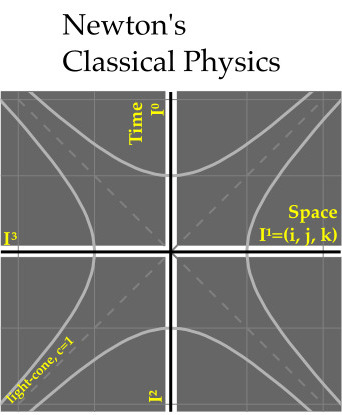
\includegraphics{../images/QM/BellsFuture/Bells_future_QM_Newton.jpg}

Space is abosulte. Time is absolute. There is no way in Newtonian
physics to rotate space into time. This is the physics we experience
everyday.

\hypertarget{einsteins-causal-relativistic-physics}{%
\subsection{Einstein's Causal Relativistic
Physics}\label{einsteins-causal-relativistic-physics}}

The only kinds of events that can change an observer at the origin are
events from the past lightcone.

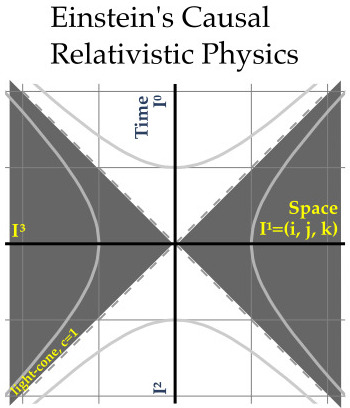
\includegraphics{../images/QM/BellsFuture/Bells_future_QM_Einstein.jpg}

Einstein was adroit at working with the space-like regions, realizing
for example that events that are simultaneous in one reference frame
will not be so in another. If one decides to restrict to the study
causality, that is the reason to black out the space-time regions. Why
did something happen? The answer is in the past lightcone, not the
space-like region.

\hypertarget{bells-future-quantum-mechanics}{%
\subsection{Bell's Future Quantum
Mechanics}\label{bells-future-quantum-mechanics}}

This is from a
\href{https://en.wikipedia.org/wiki/EPR_paradox\#The_paradox}{Wikipedia
discussion of EPR paper}:

\begin{verbatim}
The 1935 EPR paper condensed the philosophical discussion into a physical argument. The authors claim that given a specific experiment, in which the outcome of a measurement is known before the measurement takes place, there must exist something in the real world, an "element of reality", that determines the measurement outcome. They postulate that these elements of reality are, in modern terminology, local, in the sense that each belongs to a certain point in spacetime. Each element may, again in modern terminology, only be influenced by events which are located in the backward light cone of its point in spacetime (i.e., the past).  These claims are founded on assumptions about nature that constitute what is now known as local realism.
\end{verbatim}

It was the clause ``only be influenced by events which are located in
the backward light cone'' that caught my attention. If there are no
hidden variables as shown by experiments, remove any possibility.

Notice how Einstein causality and Bell's future combine to cover all of
space-time. Both relativity and quantum mechanics were born and matured
in the same time window, and at for Einstein, in the same mind.

\hypertarget{repeat-the-exercise-for-tangent-spaces}{%
\subsection{Repeat the Exercise for Tangent
Spaces}\label{repeat-the-exercise-for-tangent-spaces}}

Space-time records where-when things are: location, location, location.
Space-time formally has no information about change. Change lives in
tangent spaces. Which tangent space is used determines what change is
under study. The most common one is energy-momentum. Tangent spaces can
also be broken up into the same four types: all, classical,
relativistic, and quantum:

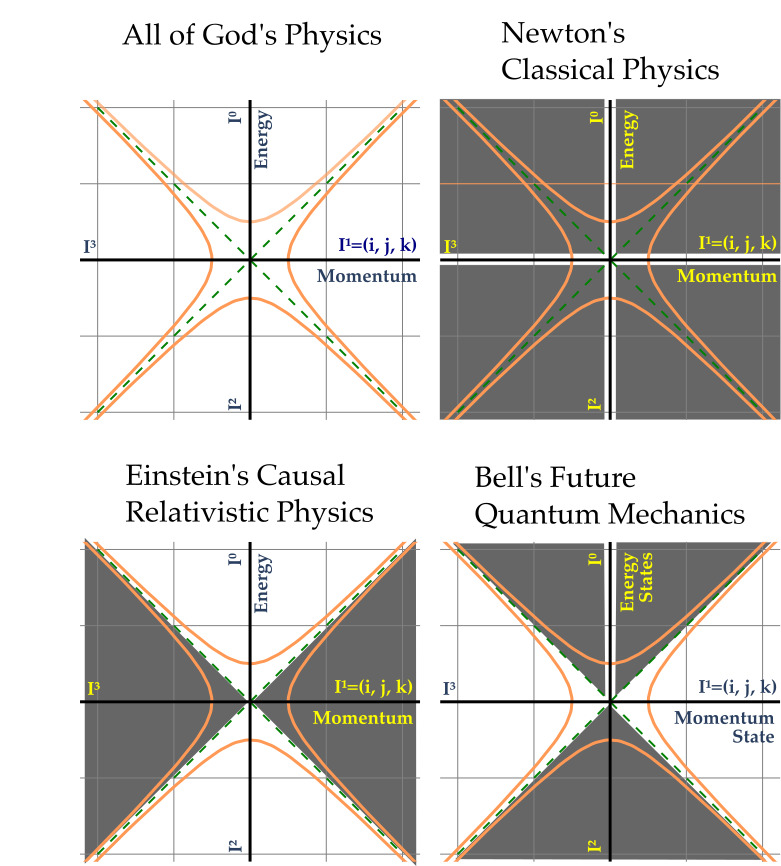
\includegraphics{../images/QM/BellsFuture/Bells_future_EP.jpg}

Imagine one were to study the classical motion of a rock. There would be
energy and momentum at the point in space-time where the rock happened
to be. Everywhere-when else in space-time, the energy-momentum space
would be zero. These zeroes are usually ignored, so the topic of tangent
spaces only appears at the graduate-level. It makes the switch to
continuous fields seem mystical. Instead, the difference between the two
is more like discrete and continuous for energy-momentum.

Physicists have studied all combinations of the base space space-time
with the tangent space energy-momentum. There is both classical and
relativistic quantum mechanics.

\hypertarget{uncool-sidebar-the-base-space-is-the-base}{%
\subsubsection{Uncool Sidebar: The Base Space is the
Base}\label{uncool-sidebar-the-base-space-is-the-base}}

The base space, space-time, cannot be changed by anything. I appreciate
that this clear statement will be violently rejected by those who have
made a serious study of Einstein's general relativity. Tens of thousands
of times it has been repeated: gravity bends space-time. I am not in
denial of the words. I do feel compelled to at least question the link
to the math. Gravity alters a tangent space of space-time as seen by the
dt and dR in metric solutions. Space-time has Lorentz symmetry and its
origin. Gravity and energy-momentum have Poincare symmetry. Summing up
all the changes in all the tangent spaces results in a curved path in
space-time. All the change happens in the tangent space. We should be
saying the tangent space is curved then summed, not that the base space
is curved.

End sidebar

\hypertarget{momentum-versus-a-momentum-state}{%
\subsection{Momentum versus a Momentum
State}\label{momentum-versus-a-momentum-state}}

Why use momentum in relativity, but momentum states in quantum
mechanics? Momentum from the past lightcone can change the motion of the
observer at the origin. The entire chain of events leading to that chang
in the observer can be known. A space-like momentum state is different.
Momentum states may never change the observer at the origin, here-now.
The precise odds of a momentum state changing the momentum of an
observer can be calculated. In the future, if an interaction does occur,
it will change the path of the observer in the usual way. The entire
chain of events leading to this momentum change cannot be known because
they are space-like separated. The observer is necessarily blind-sided
by a momentum state.

The same story applies to energy versus an energy state. Observers can
absorb energy from the past lightcone and heat up. Observers cannot
absorb energy from an energy state as it is too far away. The can in the
futur absorb the energy to the same effect. We can calculate the odds.

\hypertarget{the-wave-function}{%
\subsection{The Wave Function}\label{the-wave-function}}

The wave function is a set of space-like energy-momentum states. Each
state may not have a time-like relationship to the observer at the
origin, here-now. Each state of the wave function can have a time-like
relationship with other states in the wave function. Light-like
relationships are not addressed for the moment as that is a refinement
one will have to include with care later.

For a complex-valued wave function, the conjugate is simple to
construct. The product of a wave function and its conjugate evaluates to
a positive real number. If properly normalized, the postive number is
the odds of an interation happening. Nothing unusual is happening under
the Bell's future interpretation, all calculations will be the same.

\hypertarget{dull-quaterion-series-quantum-mechanics}{%
\subsection{Dull Quaterion Series Quantum
Mechanics}\label{dull-quaterion-series-quantum-mechanics}}

Quaternion quantum mechanics has been studied and presented in a
book-length form by Stephen Adler. The topic has been commented on in a
December 2018 blog by Scott Aaronson where he came to the conclusion
that quaternion quantum mechanics was a ``complete dumpster fire''
because it would allow superluminal transfer of information. I agree,
any algebraic system that allows superluminal transformation is boring
and deserves no futher study. I was suprised that this flaw was known to
Adler as he admitted to Aaronson.

In a rapid exchange I had with Aaronson, I came up with the idea of
``point-one-way'' quaternions. Pick an arbitrary direction and stick
with that for all calculations. Aaronson agreed it would work. He just
thought it was so dull it did not even deserve a new name.

As I considered it more, a better name would have been
``point-with-precision'' quaternion series quantum mechanics. In the
lab, physics experiments are reknown for their precision of the
experimental apperatus. It is common to use tables that isolate the
vibrations of the surroundings from the experiment. The precision of
location known at the bench is apply to the math used. Quaternions that
point in the same direction commute. A quaternion series is not a
division algebra like the quaternions. Instead it is a semi-group with
inverses. A semi-group has more than one inverse.

For quaternion-valued wave functions, the conjugate has a physical
meaning: it is a mirror reflection in space. Why do so? The product of
the wave function and its mirror reflection is a here-future value, (0,
0, 0) for the 3-vector and a positive real number. If properly
normalized, the real value is the odds of seeing an interaction. It is
the simple, physical interpretation of an otherwise abstraction notion
of a complex-valued wave function that I see as a benefit worthy of
exploration.

The Bell's future quantum mechanics interpretation in no way depends on
quaternion series quantum mechanics being a viable algebric approach to
doing calculations.

\hypertarget{interpretations-of-quantum-mechanics}{%
\subsection{Interpretations of Quantum
Mechanics}\label{interpretations-of-quantum-mechanics}}

There are at least 20 intepretations of quantum mechanics. Nearly all of
them make the same predictions as does this one. I have seen Sean
Carroll take a poll of graduate students to find their favorite. This is
not the was physics works. Physics is a contact sport with only one
eventual winner.

Physics by subtraction defines areas of study. Newton's classical
physics uses only the axes. Causality in special relativity uses only
the past lightcone. By contrast, quantum mechancis uses nothing from the
past lightcone. Quantum mechanics uses space-like states to calculate
the odds of interactions in the future.

Bell's future quantum mechanics looks bright. I hope this idea goes
viral in a good way.
